\begin{card}
	\frametitle{Übung 3: Paradigmen}
	\url{http://people.f4.htw-berlin.de/~hebold/htw/pka/exercises/konzepte-Paradigmen.pdf}
\end{card}

\begin{card}
	Das von-Neumann-Rechnerkonzept (auch von-Neumann-Architektur) zählt zur archetypischen Realisierung des imperativen Programmierparadigmas. Warum?
	\hr
	Imperative Konzept $\ent$ Befehlsorientiert\\
	Fetch, Execute-Zyklus
\end{card}

\begin{card}
Die Turing-Maschine realisiert ebenfalls das imperativen Programmierparadigma. Warum?
\hr
Jeder Zustand verknüpft über Befehle, vgl. Überführungsfunktion
\end{card}

\begin{card}
	Wiese wird vom von-Neumann-Rechner\textbf{konzept} aber von der Turing-\textbf{Maschine} gesprochen?
	\hr
	Konzept: Abstraktion
	
	Maschine: Konkrete Idee (auch wenn so nicht realisierbar)
	\begin{figure}[h]
	\centering
	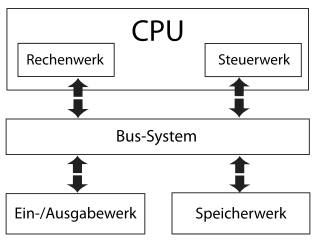
\includegraphics[width=4cm]{Von-Neumann_Architektur}
	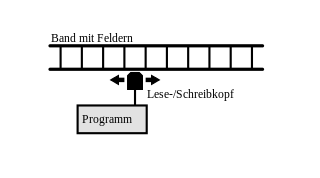
\includegraphics[width=6cm]{Turingmaschine}
	\caption{Von-Neumann, Turing-Maschine}
	\end{figure}
\end{card}

\begin{card}
	Im Zusammenhang mit dem Neumann-Rechnerkonzept ist die Rede vom von-Neumann-Flaschenhals, wenn Nachteile des Konzepts genannte werden.
	
	\hr
	a) Was ist darunter zu verstehen?
	
	Alle Befehle müssen durch den Bus
	\hr
	b) Gibt es eine vergleichbare Problematik für die Turing-Maschine? 
	
	Schreib/Lesekopf kann nur entweder schreiben oder lesen
\end{card}

\begin{card}
	Nennen Sie wenigstens einen konzeptionellen Unterschied zwischen von-Neumann-Rechnerkonzept und Turing-Maschine.
	\hr
	Von TM ausgehend:
	
	\begin{enumerate}
	\item Daten und Programme liegen \textbf{nicht} im selben Speicher
	\item keine Nummerierung auf dem Band
	\item keine Sprungadressen
	\item kann nur 1 Feld gehen pro Befehl
	\end{enumerate}
\end{card}

\begin{card}
	Setzt die Turing-Maschine das von-Neumann-Rechnerkonzept um?
	\hr
	\textbf{Nein}, weil
	\begin{enumerate}
	\item Bei TM: Daten $\neq$ Programme
	\item TM hat keine Sprungadresse
	\end{enumerate}
	oder \textbf{Ja} mit Einschränkungen (s.o)
\end{card}

\begin{card}
	Wie könnte das Paradigma der strukturierten Programmierung in das von-Neumann-Rechnerkonzept integriert werden?
	\hr
	Überwachen, bzw. Regeln der Sprunganweisungen.\\
	D.h. Begrenzter Bereich z.B. bei if-Anweisungen
\end{card}

\begin{card}
	Wieso verletzt das Konzept der lokalen static-Variablen in C das Paradigma der funktionalen
	Programmierung?
	\hr
	Funktionsausgabe nur abhängig von Eingabe. D.h. bei gleicher Eingabe gleiche Ausgabe.
	\begin{lstlisting}[language=C]
int f(int i) {
  // Ausfuehrung bei Objekt-Init, 
  // nicht bei Methodenaufruf
  static int x = 0; 
  x++;
  return x+i;
}
	\end{lstlisting}	
\end{card}

\begin{card}
	Wieso verletzen Pointer in C das Paradigma der funktionalen Programmierung?
	\hr
	Pardigma der f. Programmierung: Funktionsausgabe nur abhängig von Eingabe.  D.h. bei gleicher Eingabe gleiche Ausgabe.
	\begin{lstlisting}[language=C]
int f(int *i) {
  // Veraendern der Speicheradresse und 
  //somit der Eingabe
  *i = 1234
  ...
}
	\end{lstlisting}	
\end{card}

\begin{card}
	In Java gibt es mit dem Collection-Framework eine Reihe von sogenannten Container-Klassen. Welches objektorientierte Programmierparadigma verletzen Objekte z.B. der Klassen	ArrayList oder Vector? 
	\hr
	Es werden Referenzen gespeichert. D.h. die Datenkapselung ist verletzt.
	\begin{lstlisting}[language=Java]
Class Dummy{int value;}
...
Dummy example = new Dummy()
ArrayList<Dummy> list = new ArrayList<Dummy>()
list.add(example)

// Zugriff auf value via:
example.value
list.get(0).value
	\end{lstlisting}	
\end{card}

\begin{card}
	Wie müsste das Funktionskonzept in C beschränkt bzw. erweitert werden, damit es nicht zu Verletzungen des Paradigmas der funktionalen Programmierung kommen kann?
	\hr
	\begin{enumerate}
	\item kein static und Pointer 
	\item keine Systemaufrufe
	\end{enumerate}
\end{card}

\begin{card}
	Das funktionale Programmierparadigma, das die referentielle Transparenz der Variablen fordert, wird in C durch die Zuweisung verletzt. Wie müssten die Regeln für die Verwendung der Zuweisung geändert werden, damit die	Zuweisung in das funktionale Konzept passt? 
	\hr
	Welcher Art von Anweisung entspräche die veränderte Zuweisung dann? 
	TODO
\end{card}

\begin{card}
	Die referentielle Transparenz sorgt dafür, dass Programme in rein funktionalen Sprachen	problemlos nebenläufig abgearbeitet werden können. 
	Erklären Sie den Zusammenhang an einem Beispiel.
	Erklären Sie an einem Beispiel den Zusammenhang fehlender referentieller Transparenz und Problemen bei nebenläufig ausgeführten Programmen. 
\end{card}

\begin{card}
	Objektorientierte Sprachen kennen sogenannte inline-Funktionen.
	Wieso sind inline-Funktionen in objektorientierten Programmiersprachen implementiert?
	Sind inline-Funktionen in rein funktionalen Programmiersprachen sinnvoll?
	Welches Problem ergibt sich aus inline-Funktionen im Rahmen einer rein funktionalen	Sprache? 
\end{card}

\begin{card}
	Angenommen in C würden innerhalb von parametrisierten Makros Zuweisungen nicht mehr	zugelassen.	Inwiefern verletzen Makros dann trotzdem weiterhin Paradigmen der funktionalen Programmierung? 
\end{card}